\documentclass[10pt,utf8]{beamer}
\usepackage[T1]{fontenc}
\usepackage[utf8]{inputenc}
\usepackage[russian]{babel}
\usepackage[normalem]{ulem}
\usepackage{multicol}

% \usepackage{lmodern}
\usetheme{Dresden}
\usecolortheme{beaver}
% \useoutertheme{shadow}

\definecolor{links}{HTML}{2A1B81}
\hypersetup{colorlinks,linkcolor=,urlcolor=links}

\title{ReactJS\\ или\\ Как я перестал бояться и полюбил JavaScript}
\date{Anadea Inc. 19 декабря 2014}
\author{Андрей Кутейко}

\titlegraphic{
\includegraphics[scale=0.2]{react-logo.png}}

\begin{document}

\begin{frame}
  \titlepage
\end{frame}

\begin{frame}[fragile]
  \frametitle{Простейшее приложение}
  \framesubtitle{Vanilla JS}

  \begin{semiverbatim}
    <!DOCTYPE html>
    <div id="app"\phantom{}></div>
    <script>
    // создание DOM-узла
    var a = document.createElement("a");
    a.setAttribute("href"\phantom{}, "http://anadea.info");
    a.value = "Click me";

    // вставка в страницу
    document.getElementById("app").appendChild(a);
    </script>
  \end{semiverbatim}
\end{frame}

\begin{frame}[fragile]
  \frametitle{Простейшее приложение}
  \framesubtitle{ReactJS}

  \begin{semiverbatim}
    <!DOCTYPE html>
    <div id="app"\phantom{}></div>
    <script>
    // создание DOM-узла
    var a = React.createElement("a"\phantom{},
      \{href: "http://anadea.info"\},
      "Click me");

    // вставка в страницу
    React.render(a, document.getElementById("app"));
    </script>
  \end{semiverbatim}
\end{frame}

\begin{frame}[fragile]
  \frametitle{Простейшее приложение}
  \framesubtitle{createElement}

  \begin{itemize}
  \item
    \begin{semiverbatim}
React.createElement(\alert{<element>}[, \alert{<properties>}
  [, \alert{<children>...}]])
    \end{semiverbatim}
    \pause

  \item
    \begin{semiverbatim}
React.DOM.\alert{<element>}([\alert{<properties>}[, \alert{<children>...}]])
    \end{semiverbatim}
    \pause

  \item
    \begin{semiverbatim}
\alert{<element factory>}([\alert{<properties>}[, \alert{<children>...}]])
    \end{semiverbatim}
  \end{itemize}
\end{frame}

\begin{frame}[fragile]
  \frametitle{Простейшее приложение}
  \framesubtitle{DOM factory}

  \begin{semiverbatim}
    <!DOCTYPE html>
    <div id="app"\phantom{}></div>
    <script>
    React.render(
      \alert{React.DOM.a}(\{href: "http://anadea.info"\}, "Click me"),
      document.getElementById("app"));
    </script>
  \end{semiverbatim}
\end{frame}

\begin{frame}[fragile]
  \frametitle{Простейшее приложение}
  \framesubtitle{Класс}

  \begin{semiverbatim}
    var SimpleApp = React.createClass(\{
      render: function() \{
        \alert{return React.DOM.a(
          \{href: "http://anadea.info"\},
          React.DOM.img(\{src: "/assets/logo.png"\}),
          "Click me"
        );}
      \}
    \});

    React.render(
      \alert{React.createElement(SimpleApp)},
      document.getElementById("app"));
  \end{semiverbatim}
\end{frame}

\begin{frame}[fragile]
  \frametitle{Простейшее приложение}
  \framesubtitle{Свойства}

  \begin{semiverbatim}
    var SimpleApp = React.createClass(\{
      render: function() \{
        return React.DOM.a(
          \{href: \alert{this.props.url}\},
          React.DOM.img(\{src: "/assets/logo.png"\}),
          \alert{this.props.title}
        );
      \}
    \});

    React.render(
      React.createElement(SimpleApp,
        \alert{\{url: "http://anahoret.com"\phantom{},
         title: "Жми!"\}}),
      document.getElementById("app"));
  \end{semiverbatim}
\end{frame}

\begin{frame}[fragile]
  \frametitle{Элементарное приложение}
  \framesubtitle{Ссылки и события}

  \begin{semiverbatim}
    var ElementaryApp = React.createClass(\{
      render: function() \{
        return React.DOM.div(null,
          React.DOM.input(\{\alert{ref: "inp"}\}),
          React.DOM.a(
            \{href: "\phantom{}"\phantom{}, onClick: \alert{this.onClick}\},
            this.props.title
          )
        );
      \},
      onClick: function(event) \{
        event.preventDefault();
        document.location = \alert{this.refs.inp.getDOMNode()}.value;
      \}
    \});
  \end{semiverbatim}
\end{frame}

\begin{frame}[fragile]
  \frametitle{Элементарное приложение}
  \framesubtitle{Компонент}

  \fontsize{9pt}{9.2}\selectfont

  \begin{semiverbatim}
    var \alert{Button} = React.createClass(\{
      getDefaultProps: function() \{
        return \{ title: "Button1"\phantom{},
                 onClick: function() \{\} \};
      \},
      render: function() \{
        React.DOM.a(\{ href: "\phantom{}"\phantom{},
                      className: "btn"\phantom{},
                      onClick: this.onClick \},
          this.props.title);
      \},
      onClick: function(event) \{
        event.preventDefault();
        this.props.onClick();
      \}
    \});
  \end{semiverbatim}
\end{frame}

\begin{frame}[fragile]
  \frametitle{Элементарное приложение}
  \framesubtitle{Компонент (cont.)}

  \begin{semiverbatim}
    var ElementaryApp = React.createClass(\{
      render: function() \{
        return React.DOM.div(null,
          React.DOM.input(\{ref: "inp"\}),
          \alert{React.createElement(Button,
            \{ title: this.props.title,
              onClick: this.onButtonClick \})}
        );
      \},
      onButtonClick: function() \{
        document.location = this.refs.inp.getDOMNode().value;
      \}
    \});
  \end{semiverbatim}
\end{frame}

\begin{frame}[fragile]
  \frametitle{Элементарное приложение}
  \framesubtitle{Состояние}

  \fontsize{9pt}{9.2}\selectfont

  \begin{semiverbatim}
    var ElementaryApp = React.createClass(\{
      getInitialState: function() \{
        return \{ \alert{url: "\phantom{}"} \};
      \},
      render: function() \{
        return React.DOM.div(null,
          React.DOM.input(\{ onChange: this.onUrlChange,
                            value: \alert{this.state.url} \}),
          React.createElement(Button, \{ onClick: this.onButtonClick \})
        );
      \},
      onUrlChange: function(event) \{
        \alert{this.setState(\{url: event.target.value\});}
      \},
      onButtonClick: function(event) \{
        document.location = \alert{this.state.url};
      \}
    \});
  \end{semiverbatim}
\end{frame}

\begin{frame}[fragile]
  \frametitle{Примитивное приложение}
  \framesubtitle{Состояние}

  \begin{semiverbatim}
    var CounterApp = React.createClass(\{
      getInitialState: function() \{
        return \{ \alert{count: 0} \};
      \},
      render: function() \{
        return React.createElement(Button,
          \{ onClick: this.onClick \},
          \alert{this.state.count}
        );
      \},
      onClick: function() \{
        this.setState(\{\alert{count: this.state.count + 1}\});
      \}
    \});
  \end{semiverbatim}
\end{frame}

\begin{frame}[fragile]
  \frametitle{Как всё это работает}
  \framesubtitle{Из чего состоит компонент}

  \begin{itemize}
  \item
    Render function
    \pause
  \item
    Properties \\
    Children -- это тоже свойство
    \pause
  \item
    State
    \pause
  \item
    Любые пользовательские методы
  \end{itemize}
\end{frame}

\begin{frame}[fragile]
  \frametitle{Жизненный цикл компонентов}

  \begin{itemize}
  \item Вставка (mounting)

    getInitialState \\
    componentWillMount \\
    componentDidMount

    \pause

  \item Обновление (updating)

    componentWillReceiveProps \\
    shouldComponentUpdate \\
    componentWillUpdate \\
    componentDidUpdate

    \pause

  \item Удаление (unmounting)

    componentWillUnmount
  \end{itemize}
\end{frame}

\begin{frame}[fragile]
  \frametitle{Как всё это работает}

  \begin{itemize}
  \item
    Что происходит
    $$ (props \times state) \rightarrow Virtual DOM \rightarrow DOM $$
    \pause
  \item
    Что делает наш код
    $$ \alert{ (props \times state) \rightarrow Virtual DOM } \rightarrow DOM $$
    \pause
  \item
    Что на себя берёт ReactJS
    $$ (props \times state) \rightarrow \alert{ Virtual DOM \rightarrow DOM } $$
  \end{itemize}
\end{frame}

\begin{frame}[fragile]
  \frametitle{Как всё это работает}
  \framesubtitle{Virtual DOM (1)}

  \begin{semiverbatim}
    React.DOM.a(\{href: "/"\}, "Home")
  \end{semiverbatim}

  \begin{semiverbatim}
    \{
      "name": "a"\phantom{},
      "attrs": \{"href": "/"\},
      "children": ["Home"]
    \}
  \end{semiverbatim}
\end{frame}

\begin{frame}[fragile]
  \frametitle{Как всё это работает}
  \framesubtitle{Virtual DOM (2)}

  \begin{semiverbatim}
    React.createElement(Button)
  \end{semiverbatim}

  \begin{semiverbatim}
    \{
      "name": "a"\phantom{},
      "attrs": \{
        "href": "\phantom{}"\phantom{},
        "class": "btn"
      \},
      "children": [
        "Button1"
      ]
    \}
  \end{semiverbatim}
\end{frame}

\begin{frame}[fragile]
  \frametitle{Как всё это работает}
  \framesubtitle{Virtual DOM (3)}

  \fontsize{9pt}{9.2}\selectfont

  \begin{semiverbatim}
    React.DOM.div(null,
      React.DOM.input(\{value: "http://anadea.info/"\}),
      React.createElement(Button))
  \end{semiverbatim}

  \begin{semiverbatim}
    \{
      "name": "div"\phantom{},
      "attrs": \{\},
      "children": [
        \{
          "name": "input"\phantom{},
          "attrs": \{ "value": "http://anadea.info/" \},
          "children": []
        \},
        \{
          "name": "a"\phantom{},
          "attrs": \{ "href": "\phantom{}"\phantom{}, "class": "btn" \},
          "children": [ "Button1" ]
        \}
      ]
    \}
  \end{semiverbatim}
\end{frame}

\begin{frame}[fragile]
  \frametitle{Как всё это работает}
  \framesubtitle{Data flow}

  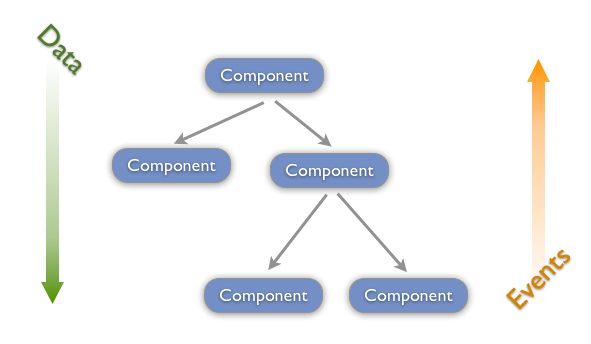
\includegraphics[scale=0.5]{data-event-flow.png}
\end{frame}

\begin{frame}[fragile]
  \frametitle{Grok ReactJS}
  \framesubtitle{Состояние не нужно}

  \fontsize{9pt}{9.2}\selectfont

  \begin{semiverbatim}
List = React.createClass
  render: ->
    React.DOM.ul null,
      \alert{@props.children}.map (child, index) =>
        React.DOM.li \{ key: index \},
          \alert{child},
          Button \{onClick: \alert{@props.onDeleteItem}.bind(null, index)\}, "X"


App = React.createClass
  render: ->
    React.createElement List, \{ onDeleteItem: @onDeleteItem \},
      @state.items.map (item) ->
        React.createElement \alert{Widget}, \{ data: item \}

  onDeleteItem: (index) ->
    items = @state.items.slice().splice(index, 1)
    @setState \{ items: items \}
  \end{semiverbatim}
\end{frame}

\begin{frame}[fragile]
  \frametitle{Grok ReactJS}
  \framesubtitle{Состояние не нужно}

  \fontsize{8pt}{8.2}\selectfont

  \begin{semiverbatim}
List = React.createClass
  render: ->
    React.DOM.ul null,
      \alert{@props.items}.map (item, index) =>
        React.DOM.li key: index,
          \alert{@props.createItem}(item),
          Button \{ onClick: @onDelete.bind(null, index) \}, "X"

  onDelete: (index) ->
    children = @props.items.slice().splice(index, 1)
    @props.onChangeItems children

App = React.createClass
  render: ->
    React.createElement List,
      items: @state.\alert{items}
      createItem: (item) ->
        React.createElement \alert{Widget}, {data: item}
      onChangeItems: @onChangeItems

  onChangeItems: (items) ->
    @setState {items: items}
  \end{semiverbatim}
\end{frame}

\begin{frame}[fragile]
  \frametitle{Code reuse}
  \framesubtitle{Миксины}

  \fontsize{9pt}{9.2}\selectfont

  \begin{semiverbatim}
var UndoStack = \{
  getInitialState: function() \{
    return \{ undo: [] \};
  \},
  snapshot: function() \{
    var undo = this.state.undo.concat(\alert{this.getStateSnapshot()});
    this.setState(\{ undo: undo \});
  \},
  undo: function() \{
    var undo = this.state.undo.slice();
    var snapshot = undo.pop();
    \alert{this.setStateSnapshot(snapshot)};
    this.setState(\{ undo: undo \});
  \}
\};

var MyComponent = React.createClass(\{
  mixins: [ UndoStack ],
  getStateSnapshot: function() \dots
  setStateSnapshot: function(snapshot) \dots
  \end{semiverbatim}
\end{frame}

\begin{frame}[fragile]
  \frametitle{JSX}

  \fontsize{9pt}{9.2}\selectfont

  \begin{semiverbatim}
    /** @jsx React.DOM */

    var SimpleApp = React.createClass(\{
      \dots
      render: function() \{
        return \alert{<div>
          <input onChange=}\{this.onUrlChange\} \alert{value=}\{this.state.url\}\alert{>
          <Button onClick=}\{this.onButtonClick\}\alert{>
        </div>;}
      \},
      \dots
    \});
  \end{semiverbatim}
\end{frame}

\begin{frame}[fragile]
  \frametitle{Разное}

  \begin{itemize}
  \item CSS, SVG, Canvas\dots
    \pause
  \item Синтетические события
    \pause
  \item Модульные тесты $(props \times state) \rightarrow Virtual DOM$
    \pause
  \item Server-side rendering
    \pause
  \item Immutable.js
  \end{itemize}
\end{frame}

\begin{frame}[fragile]
  \frametitle{Альтернативы}

  \begin{center}
    
\includegraphics[scale=0.3]{alternatives.jpg}
  \end{center}
\end{frame}

\begin{frame}[fragile]
  \frametitle{Ссылки}

  \begin{enumerate}
  \item \href{http://facebook.github.io/react/}{http://facebook.github.io/react/}
  \item \href{https://github.com/andy128k/reactjs-presentation}{https://github.com/andy128k/reactjs-presentation}
  \item \href{https://github.com/facebook/immutable-js}{https://github.com/facebook/immutable-js}
  \end{enumerate}
\end{frame}

\begin{frame}[fragile]
  \frametitle{Вопросы?}

  \begin{center}
    
\includegraphics[scale=0.25]{strangelove.png}
  \end{center}
\end{frame}

\end{document}

